\id{ҒТАМР \href{https://grnti.ru/?p1=52&p2=47&p3=01}{52.47.01}}

\begin{articleheader}
\sectionwithauthors{Б.М. Нұранбаева}{МҰНАЙ ЖӘНЕ ГАЗ КЕН ОРЫНДАРЫН КЕШЕНДІ ИГЕРУ ТИІМДІЛІГІН ТАЛДАУ}

{\bfseries Б.М. Нұранбаева}
\end{articleheader}
\begin{affiliation}
  
Caspian University, Алматы, Қазақстан

\raggedright {\bfseries \textsuperscript{\envelope }}Corresponding-author: \href{mailto:bulbulmold@mail.ru}{\nolinkurl{bulbulmold@mail.ru}}
\end{affiliation}

Қарастырлып отырған мақала қабаттан құрамында ванадий бар мұнайдың
қалдық қорларын алу мәселесіне және сұйық ортадағы ванадий иондарымен
отандық редоксполимерлердің өзара әрекет ету үрдістеріне арналған.

Мұнай және газ кен орындарын игеру және пайдалану тәсілдерін тиімділігін
талдау, Қазақстан аумағында өндірудің тиімді технологиясын пайдалану
және мұнайдан ванадий қабаттарынан мұнай өндіру қарқындылығы мен
мұнайбергіштік коэффициентін арттыру болып табылады. Мұнай мен мұнай
өнімдерінен ілеспе-өндірілетін ванадий, сонымен қатар, газ кен орындарын
әзірлеу кезінде газды (гелий және т.б.) алудың инновациялық тәсілі
ұсынылған, бұл әдіс мұнай-газ саласына отандық редоксполимерлер
негізінде мұнай мен мұнай өнімдерінен ванадий мен басқа да металдарды
алу үшін сорбциялық процестерді, сондай-ақ, газдарды бөлу кезінде
мембраналық технологияны енгізу, бұл мұнай және газ кен орындарын
кешенді игеру талаптарына сәйкес, мұнай газының сапасын және оны өндіру
орнынан тұтынушыға дейін тасымалдау тиімділігін арттыру.

Мақалада қарастырылған талдау іске асыру қалдықтарды кәдеге жарату
бойынша қазіргі заманның бірқатар табиғат қорғау міндеттерін шешуге,
республиканың мұнай өндіру және мұнай өңдеу өңірлеріне техногендік
экологиялық жүктемені азайтуға мүмкіндік береді.

{\bfseries Түйін сөздер:} кен орын, пайдалы қазбалар, талдау, технологиялық
сұлба.

\begin{articleheader}
{\bfseries АНАЛИЗ ЭФФЕКТИВНОСТИ КОМПЛЕКСНОГО ОСВОЕНИЯ МЕСТОРОЖДЕНИЙ НЕФТИ И ГАЗА}

{\bfseries Б.М. Нуранбаева}
\end{articleheader}
\begin{affiliation}

Caspian University, Алматы, Казахстан,

e-mail: \href{mailto:bulbulmold@mail.ru}{\nolinkurl{bulbulmold@mail.ru}}
\end{affiliation}

Рассматриваемая статья посвящена проблеме извлечения остаточных запасов
ванадийсодержащей нефти из пласта и процессам взаимодействия
отечественных редоксполимеров с ионами ванадия в жидких средах.

Анализ эффективности методов разработки и эксплуатации месторождений
нефти и газа, использования эффективной технологии добычи на территории
Казахстана и повышения интенсивности добычи нефти из ванадиевых пластов
и коэффициента нефтеотдачи. Предложен инновационный способ к получению
попутно добываемого ванадия из нефти и нефтепродуктов, а также газа
(гелия и др.) при разработке газовых месторождений, способ которого
заключается в внедрении в нефтегазовую отрасль сорбционных процессов для
извлечения ванадия и других металлов из нефти и нефтепродуктов на основе
отечественных редоксполимеров, а также мембранной технологии при
разделении газов это в соответствии с требованиями комплексного освоения
нефтегазовых месторождений, повышения качества нефтяного газа и
эффективности его транспортировки от места добычи к потребителю.

Реализация рассмотренного в статье анализа позволит решить ряд
современных природоохранных задач по утилизации отходов, снизить
техногенную экологическую нагрузку на нефтедобывающие и
нефтеперерабатывающие регионы республики.

{\bfseries Ключевые слова:} месторождение, полезные ископаемые, анализ,
технологическая схема.
\begin{articleheader}

{\bfseries ANALYSING THE EFFICIENCY OF INTEGRATED DEVELOPMENT OF OIL AND GAS FIELDS}

{\bfseries B. Nuranbayeva}
\end{articleheader}
\begin{affiliation}

Caspian University, Almaty, Kazakhstan,

e-mail: \href{mailto:bulbulmold@mail.ru}{\nolinkurl{bulbulmold@mail.ru}}
\end{affiliation}

The article is devoted to the problem of extraction of residual reserves
of vanadium-containing oil from the reservoir and the processes of
interaction of domestic redoxpolymer with vanadium ions in liquid media.

Analysis of the efficiency of methods of development and operation of
oil and gas fields, the use of effective production technology in
Kazakhstan and increase the intensity of oil production from
vanadium-bearing formations and oil recovery factor. An innovative
method to obtain associated vanadium from oil and oil products, as well
as gas (helium, etc.) in the development of gas fields is proposed. The
method consists in introducing into the oil and gas industry sorption
processes for the extraction of vanadium and other metals from oil and
oil products on the basis of domestic redoxpolymers, as well as membrane
technology in the separation of gases it is in accordance with the
requirements of integrated development of oil and gas fields, improving
the quality of oil gas and the efficiency of its transmission to the oil
and gas industry.

Realisation of the analysis considered in the article will allow to
solve a number of modern environmental protection tasks on waste
utilisation, to reduce technogenic ecological load on oil producing and
oil refining regions of the republic.

{\bfseries Keywords:} field, minerals, analysis, process flowchart.
\begin{multicols}{2}

{\bfseries Кіріспе.} Әлемнің индустриалды дамыған елдерінде мұнай және
мұнай өнімдерін тұтынудың өсуі олардың бағасының тез өсуіне және
тұрақсыздығына әкелді, ал мұнайдың салыстырмалы түрде шектеулі қоры
ғалымдарды өндіру мен тұтыну саласына әлі қатыспаған көмірсутек
шикізатының жаңа үнемді көздерін іздеуге мәжбүр етеді {[}1,2{]}.

Автор {[}3{]} мұнай-газ саласындағы шолу ағымдағы әдебиеттердегі және
одан әрі зерттеу мен зерттеуді қажет ететін салалардағы елеулі
олқылықтарды, атап айтқанда, жеткізу тізбегіндегі тұрақтылықтың
экологиялық, әлеуметтік және экономикалық өлшемдерінің өзара байланысын
қарастыратын кешенді негіздің жоқтығын көрсетеді.

Автор {[}4{]} ғалымдар зерттеу мен практиктерге мұнай-газ саласындағы
жеткізу тізбегін тұрақты басқарудың кешенді перспективасын береді деп
күтілуде, яғни зерттеушілер болашақта саланы тереңірек түсінуге ықпал
етеді.

Дәстүрлі мұнай қорларының шектелуі, мұнайды тұтынудың жоғары қарқыны
және мұнай шикізаты бағасының өсуі көмірсутек шикізатының баламалы
көздерін іздеуді қажет етеді. Батыс Қазақстанда 120 м-ге дейінгі
тереңдікте 1 млрд. тоннадан астам табиғи битумдар немесе 15-20 млрд.
тоннадан астам мұнай-битуминозды жыныстар жатыр деген болжам бар. Осыған
байланысты табиғи битумдардың және тұтқырлығы жоғары мұнайлардың
көптеген қабаттары мен көкжиектері барлық жерде және үлкен тереңдікте
кездеседі.

Қазақстанның мұнай өндіру өнеркәсібінің қазіргі заманғы дамуы мұнай
қорлары құрылымының нашарлауымен сипатталады. Өндірудің тиімділігіне
қабаттардың мұнай өндірісін арттырудың жаңа технологияларын қолданған
жағдайда ғана қол жеткізуге болатын қиын қорлар барған сайын арта
бастады. Қазіргі жағдайда қиын алынатын қорлардың рөлі едәуір артып
келеді, өйткені Қазақстанның игеріліп жатқан кен орындарында мұнай
бергіштіктің тек бір пайызға артуы бойынша 2,5-3 жылдық мұнай өндіруді
қамтамасыз ете алатын бірнеше ірі кен орындарын ашуға тең.

Қазақстанның ірі кен орындарында мұнай өндірудің күрт төмендеуімен
игерудің соңғы сатысына енгенін ескере отырып, мұнай өндіруді
тұрақтандырудың және Қазақстанның мұнай өнеркәсібін одан әрі дамытудың
басты шарты өндірілуі қиын қорлары бар өнімділігі төмен қабаттардан
мұнай алуды ұлғайтудың жаңа жоғары тиімді технологиялық шешімдерін
әзірлеу және енгізу өзекті мәселе болып табылады.

Болашақта Қазақстанда мұнай мен газ өндіру көлемі айтарлықтай өсуге
ұмтылатын болады. Қазақстандық мұнай мен газ өндірісінің ұлғаюы үш
фактормен байланысты. Біріншіден, бұл инвестициялардың айтарлықтай
ағынына байланысты. Екіншіден, көмірсутек шикізатының әлемдік
нарықтарының қалыптасып келе жатқан қолайлы конъюнктурасы. Үшіншіден,
саланың ресурстық әлеуетін одан әрі арттыруға сондай-ақ, Каспий және
Арал теңіздерінің акваториясындағы жер қойнауы учаскелерін жүргізіліп
жатқан кең ауқымды зерделеу ықпал ететін болады {[}5{]}.

ХХІ ғ. Каспий өңірінің елдерін жаңа сын-қатерлерге байланысты
бұрын-соңды болмаған мүмкіндіктермен марапаттады. Каспийдің көмірсутек
ресурстарының бірінші кезектегі тұтынушысы Еуропа болып табылады, бірақ
көбінесе оған апаратын жол қиын. АҚШ энергетикалық ақпарат қызметінің
деректеріне сәйкес, Каспий өңірінде 48 млрд баррель және 8,76 трлн текше
метр газ барланған мұнай қоры бар. Каспий теңізінің қайраңы толық
зерттелмеген, континенттік қайраңның оңтүстік бөлігі Түрікменстан, Иран
және Әзірбайжан теңіз шекараларының реттелмеуіне байланысты зерттелмеген
{[}6{]}.

Қазақстан үшін Каспий мұнайы экономикалық өсуді дамыту мен қамтамасыз
етудің қуатты факторы болып табылады.

Қазіргі таңда Каспийдің әлемдік энергетика, әлемдік мұнай саясаты
жүйесіне орналасуы айқынырақ болды. Каспий Таяу Шығысқа балама бола
алмаса да, оның әлемдік энергетика үшін маңызы айтарлықтай жоғары
{[}7{]}.

Каспийдегі дәлелденген мұнай қоры шамамен 4 млрд. тоннаны құрайды.
Болжамды қорларды ескере отырып, бұл көрсеткіш әр түрлі бағалаулар
бойынша 15-тен 30 млрд.тоннаға дейін артуы мүмкін 1-кесте {[}8-9{]}.

\end{multicols}


\begin{longtable}[]{|@{}
  >{\raggedright\arraybackslash}p{(\columnwidth - 12\tabcolsep) * \real{0.1746}}|
  >{\raggedright\arraybackslash}p{(\columnwidth - 12\tabcolsep) * \real{0.1537}}|
  >{\raggedright\arraybackslash}p{(\columnwidth - 12\tabcolsep) * \real{0.1202}}|
  >{\raggedright\arraybackslash}p{(\columnwidth - 12\tabcolsep) * \real{0.1207}}|
  >{\raggedright\arraybackslash}p{(\columnwidth - 12\tabcolsep) * \real{0.1620}}|
  >{\raggedright\arraybackslash}p{(\columnwidth - 12\tabcolsep) * \real{0.1348}}|
  >{\raggedright\arraybackslash}p{(\columnwidth - 12\tabcolsep) * \real{0.1339}}|@{}}
  \caption*{1-кесте. Каспий өңіріндегі мұнай және табиғи газ қорлары} \\
\hline
Мемлекет & Дәлелденген мұнай қоры (BBL) & Мүмкін мұнай қоры (BBL) & Жалпы мұнай қорлары (BBL) & Дәлелденген газ қоры (Tcf) & Мүмкін газ қоры (Tcf) & Жалпы газ қоры (Tcf) \\ \hline
\endfirsthead
\hline
Мемлекет & Дәлелденген мұнай қоры (BBL) & Мүмкін мұнай қоры (BBL) & Жалпы мұнай қорлары (BBL) & Дәлелденген газ қоры (Tcf) & Мүмкін газ қоры (Tcf) & Жалпы газ қоры (Tcf) \\ \hline
\endhead
\hline
\endfoot
\endlastfoot
Әзірбайжан & 3,6-1,25 & 27 & 31-40 & 11 & 35 & 46 \\ \hline
Иран* & 0.1 & 12 & 12 & 0 & 11 & 11 \\ \hline
Қазақстан & 10,0-17,6 & 85 & 95-103 & 53-83 & 88 & 141-171 \\ \hline
Ресей & 0,3 & 5 & 5 & --- & --- & --- \\ \hline
Түркіменстан & 1.7 & 32 & 34 & 98-155 & 159 & 257-314 \\ \hline
Өзбекстан & 0,3 & 1 & 1 & 74-88 & 35 & 109-123 \\ \hline
Барлығы: & 16,0-32,5 & 163 & 179-195 & 236-337 & 328 & 564-665 \\ \hline
\multicolumn{7}{|@{}>{\raggedright\arraybackslash}p{(\columnwidth - 12\tabcolsep) * \real{1.0000} + 12\tabcolsep}|@{}}{%
* Ескерту - тек Каспий теңізіне жақын аймақтар.

BBL - млрд. баррель (1 баррель = 159 дм); Tcf - трл. куб фут (1 фут = 0,305 м).} \\ \hline
\end{longtable}

\begin{multicols}{2}
{\bfseries Материалдар мен әдістер.} Көмірсутектердегі ванадий мөлшері, шикізатта аз
(10\textsuperscript{-6} -дан 10\textsuperscript{-2} \%-ға дейін), ол
көптеген каталитикалық өңдеу процестеріне теріс әсер етеді.

Ванадийдің өндірісі мен оның бағасы өте аз және қарапайым түсіндіріледі.
Жер қыртысында ванадий көп болса да шамамен 0,2\% (яғни қорғасыннан 15
есе және күмістен 2000 есе көп), оның жинақталуы жерде өте сирек
кездеседі (сондықтан ванадий сирек металдарға жатады). Құрамында 1\%
ванадий бар кен өте бай болып саналады; тіпті осы құнды және тапшы
элементтің тек 0,1\% бар кендер де өнеркәсіптік өңдеуге ұшырайды.

Кендердегі ванадийдің төмен мөлшерін (максимум 1500 г/т) ескере отырып,
оның мұнай мен битумдардан ілеспе жолмен алынуы өзекті болып
есептелінеді {[}10-11{]}.

2-кестеде келтірілгендей мұнайды зерттеудегі ванадийдің еліміздегі басым
көпшік кен орындарында бар екенін көрсетеді.
\end{multicols}

\begin{longtable}[H]{|@{}
  >{\raggedright\arraybackslash}p{(\columnwidth - 6\tabcolsep) * \real{0.2681}}|
  >{\raggedright\arraybackslash}p{(\columnwidth - 6\tabcolsep) * \real{0.2537}}|
  >{\raggedright\arraybackslash}p{(\columnwidth - 6\tabcolsep) * \real{0.2732}}|
  >{\raggedright\arraybackslash}p{(\columnwidth - 6\tabcolsep) * \real{0.2050}}|@{}}
  \caption*{2-кесте. Батыс Қазақстан кен орындарының мұнай құрамындағы
ванадий мөлшері} \\
\hline
Кен орын & Құрамы, г/т & Кен орын & Құрамы, г/т \\ \hline
\endfirsthead
\hline
Кен орын & Құрамы, г/т & Кен орын & Құрамы, г/т \\ \hline
\endhead
\hline
\endfoot
\endlastfoot
\multicolumn{2}{|@{}>{\raggedright\arraybackslash}p{(\columnwidth - 6\tabcolsep) * \real{0.5217} + 2\tabcolsep}|}{\emph{Маңғыстау облысы}} &
\multicolumn{2}{|>{\raggedright\arraybackslash}p{(\columnwidth - 6\tabcolsep) * \real{0.4783} + 2\tabcolsep}|}{\emph{Ақтөбе облысы}} \\ \hline
Сол. Бозашы & 100-300 & Бозоба & 50-120 \\ \hline
Қаражанбас & 70-300 & Синельников & 5-50 \\ \hline
Қаламқас & 60-300 & Жаңажол & 1-10 \\ \hline
Жалғызтөбе & 60-200 & Кеңкияк & 1-10 \\ \hline
Қаратұрын & 70-140 & Остансук & 1-5 \\ \hline
Бесоба & 70-140 &
\multicolumn{2}{|>{\raggedright\arraybackslash}p{(\columnwidth - 6\tabcolsep) * \real{0.4783} + 2\tabcolsep}|}{\emph{Атырау облысы}} \\ \hline
Өзен & 0,5-5 & Қараарна & 40-70 \\ \hline
Асар & 0,5-5 & Тортай & 10-80 \\ \hline
Сол. Ракушечный & 0,5-5 & Құмшеті * & 10-60 \\ \hline
Жетыбай & 0,1-1 & Биікжал & 5-40 \\ \hline
Шынжыр & 0,1-1 & Теңіз & 0,1-1 \\ \hline
Тасболат & 0,05-0,5 &
\multicolumn{2}{|>{\raggedright\arraybackslash}p{(\columnwidth - 6\tabcolsep) * \real{0.4783} + 2\tabcolsep}|}{\emph{Батыс Қазақстан облысы}} \\ \hline
Оймаша & 0,01-0,1 & Гремячин & 20-50 \\ \hline
Сол. Қарагие & 0,01-0,05 & Бат. Теплов & 1-10 \\ \hline
Ұйлық & 0,001-0,01 & \multirow{3}{=}{Қарашығанақ} & \multirow{3}{=}{0,05-0,5} \\ \cline{1-2}
Жылынды & 0,001-0,01 & & \\ \cline{1-2}
Ащысор & 0,001-0,01 & & \\ \hline
\end{longtable}


% \begin{longtable}[]{@{}
%   >{\raggedright\arraybackslash}p{(\columnwidth - 6\tabcolsep) * \real{0.2681}}
%   >{\raggedright\arraybackslash}p{(\columnwidth - 6\tabcolsep) * \real{0.2537}}
%   >{\raggedright\arraybackslash}p{(\columnwidth - 6\tabcolsep) * \real{0.2732}}
%   >{\raggedright\arraybackslash}p{(\columnwidth - 6\tabcolsep) * \real{0.2050}}@{}}
% \toprule\noalign{}
% \endhead
% \bottomrule\noalign{}
% \endlastfoot
% Кен орын & Құрамы, г/т & Кен орын & Құрамы, г/т \\
% \multicolumn{2}{@{}>{\raggedright\arraybackslash}p{(\columnwidth - 6\tabcolsep) * \real{0.5217} + 2\tabcolsep}}{%
% \emph{Маңғыстау облысы}} &
% \multicolumn{2}{>{\raggedright\arraybackslash}p{(\columnwidth - 6\tabcolsep) * \real{0.4783} + 2\tabcolsep}@{}}{%
% \emph{Ақтөбе облысы}} \\
% Сол. Бозашы & 100-300 & Бозоба & 50-120 \\
% Қаражанбас & 70- 300 & Синельников & 5-50 \\
% Қаламқас & 60- 300 & Жаңажол & 1- 10 \\
% Жалғызтөбе & 60- 200 & Кеңкияк & 1- 10 \\
% Қаратұрын & 70- 140 & Остансук & 1-5 \\
% Бесоба & 70- 140 &
% \multicolumn{2}{>{\raggedright\arraybackslash}p{(\columnwidth - 6\tabcolsep) * \real{0.4783} + 2\tabcolsep}@{}}{%
% \emph{Атырау облысы}} \\
% Өзен & 0,5-5 & Қараарна & 40-70 \\
% Асар & 0,5-5 & Тортай & 10-80 \\
% Сол. Ракушечный & 0,5-5 & Құмшеті

% * & 10-60 \\
% Жетыбай & 0,1-1 & Биікжал & 5-40 \\
% Шынжыр & 0,1-1 & Теңіз & 0,1-1 \\
% Тасболат & 0,05- 0,5 &
% \multicolumn{2}{>{\raggedright\arraybackslash}p{(\columnwidth - 6\tabcolsep) * \real{0.4783} + 2\tabcolsep}@{}}{%
% \emph{Батыс Қазақстан облысы}} \\
% Оймаша & 0,01-0,1 & Гремячин & 20-50 \\
% Сол. Қарагие & 0,01-0,05 & Бат. Теплов & 1- 10 \\
% Ұйлық & 0,001-0,01 & \multirow{3}{=}{Қарашығанақ} &
% \multirow{3}{=}{0,05- 0,5} \\
% Жылынды & 0,001-0,01 \\
% Ащысор & 0,001-0,01 \\
% \end{longtable}


\begin{longtable}[]{|@{}
  >{\raggedright\arraybackslash}p{(\columnwidth - 6\tabcolsep) * \real{0.2900}}|
  >{\raggedright\arraybackslash}p{(\columnwidth - 6\tabcolsep) * \real{0.2565}}|
  >{\raggedright\arraybackslash}p{(\columnwidth - 6\tabcolsep) * \real{0.2450}}|
  >{\raggedright\arraybackslash}p{(\columnwidth - 6\tabcolsep) * \real{0.2085}}|@{}}
  \caption*{3-кесте. Батыс Қазақстан кен орындарының мұнай-битуминозды
жыныстарында ванадийдің құрамы} \\
\hline
Кен орын & Құрамы, г/т & Кен орын & Құрамы, г/т \\ \hline
\endfirsthead
\hline
Кен орын & Құрамы, г/т & Кен орын & Құрамы, г/т \\ \hline
\endhead
\hline
\endfoot
\endlastfoot
\multicolumn{2}{|@{}>{\raggedright\arraybackslash}p{(\columnwidth - 6\tabcolsep) * \real{0.5465} + 2\tabcolsep}|}{\emph{Ақтөбе облысы}} &
\multicolumn{2}{|>{\raggedright\arraybackslash}p{(\columnwidth - 6\tabcolsep) * \real{0.4535} + 2\tabcolsep}|}{\emph{Атырау облысы}} \\ \hline
Ақбұлак & 50-400 & Иманқара & 20-80 \\ \hline
Дөңгелексор & 20-70 & Ақшоқы & 10-70 \\ \hline
Мортық & 10-70 & Көлжан & 30-50 \\ \hline
Шілікті & 20-50 & Қарамұрат & 20-50 \\ \hline
Қопа & 1-20 & Мұнайлы & 10-30 \\ \hline
\multicolumn{2}{|@{}>{\raggedright\arraybackslash}p{(\columnwidth - 6\tabcolsep) * \real{0.5465} + 2\tabcolsep}|}{\emph{Маңғыстау облысы}} & \multirow{5}{=}{Қарасай} & \multirow{5}{=}{5-30} \\ \cline{1-2}
Төбежік & 10-70 & & \\ \cline{1-2}
Қарасаз-Таспас & 5-30 & & \\ \cline{1-2}
Бека-Таспас & 5-30 & & \\ \cline{1-2}
Топқараған & 1-20 & & \\ \hline
\end{longtable}
% \begin{longtable}[]{@{}
%   >{\raggedright\arraybackslash}p{(\columnwidth - 6\tabcolsep) * \real{0.2900}}
%   >{\raggedright\arraybackslash}p{(\columnwidth - 6\tabcolsep) * \real{0.2565}}
%   >{\raggedright\arraybackslash}p{(\columnwidth - 6\tabcolsep) * \real{0.2450}}
%   >{\raggedright\arraybackslash}p{(\columnwidth - 6\tabcolsep) * \real{0.2085}}@{}}
% \toprule\noalign{}
% \endhead
% \bottomrule\noalign{}
% \endlastfoot
% Кен орын & Құрамы, г/т & Кен орын & Құрамы, г/т \\
% \multicolumn{2}{@{}>{\raggedright\arraybackslash}p{(\columnwidth - 6\tabcolsep) * \real{0.5465} + 2\tabcolsep}}{%
% \emph{Ақтөбе облысы}} &
% \multicolumn{2}{>{\raggedright\arraybackslash}p{(\columnwidth - 6\tabcolsep) * \real{0.4535} + 2\tabcolsep}@{}}{%
% \emph{Атырау облысы}} \\
% Ақбұлак & 50- 400 & Иманқара & 20-80 \\
% Дөңгелексор & 20-70 & Ақшоқы & 10-70 \\
% Мортық & 10-70 & Көлжан & 30-50 \\
% Шілікті & 20-50 & Қарамұрат & 20-50 \\
% Қопа & 1-20 & Мұнайлы & 10-30 \\
% \multicolumn{2}{@{}>{\raggedright\arraybackslash}p{(\columnwidth - 6\tabcolsep) * \real{0.5465} + 2\tabcolsep}}{%
% \emph{Маңғыстау облысы}} & \multirow{5}{=}{Қарасай} &
% \multirow{5}{=}{5-30} \\
% Төбежік & 10-70 \\
% Қарасаз- Таспас & 5-30 \\
% Бека- Таспас & 5-30 \\
% Топқараған & 1-20 \\
% \end{longtable}

Тек мұнайда ғана емес, сонымен қатар, битумдарда, тақтатастарда
микроэлементтердің әртүрлі түрлері бар. Осы өнімдердегі ванадийдің
концентрациясы 3 және 4-кестеде келтірілген.


\begin{longtable}[H]{|@{}
  >{\raggedright\arraybackslash}p{(\columnwidth - 6\tabcolsep) * \real{0.2586}}|
  >{\raggedright\arraybackslash}p{(\columnwidth - 6\tabcolsep) * \real{0.2576}}|
  >{\raggedright\arraybackslash}p{(\columnwidth - 6\tabcolsep) * \real{0.2596}}|
  >{\raggedright\arraybackslash}p{(\columnwidth - 6\tabcolsep) * \real{0.2242}}|@{}}
  \caption*{4-кесте. Оңтүстік Қазақстандағы көміртекті тақтатастарындағы кен
орындарының ванадий мөлшері} \\
\hline
Кен орын & Құрамы, г/т & Кен орын & Құрамы, г/т \\ \hline
\endfirsthead
\hline
Кен орын & Құрамы, г/т & Кен орын & Құрамы, г/т \\ \hline
\endhead
\hline
\endfoot
\endlastfoot
Көксу & 500-1200 & Каратальская Долина & 50-200 \\ \hline
Шығ. Текелі алқабы & 150-300 & Кюелы & 50-250 \\ \hline
Яблонов & 80-300 & Коккус & 50-100 \\ \hline
\end{longtable}

% \begin{longtable}[]{@{}
%   >{\raggedright\arraybackslash}p{(\columnwidth - 6\tabcolsep) * \real{0.2586}}
%   >{\raggedright\arraybackslash}p{(\columnwidth - 6\tabcolsep) * \real{0.2576}}
%   >{\raggedright\arraybackslash}p{(\columnwidth - 6\tabcolsep) * \real{0.2596}}
%   >{\raggedright\arraybackslash}p{(\columnwidth - 6\tabcolsep) * \real{0.2242}}@{}}
% \toprule\noalign{}
% \endhead
% \bottomrule\noalign{}
% \endlastfoot
% Кен орын & Құрамы, г/т & Кен орын & Құрамы, г/т \\
% Көксу & 500-1200 & Каратальская Долина & 50-200 \\
% Шығ. Текелі алқабы & 150-300 & Кюелы & 50-250 \\
% Яблонов & 80-300 & Коккус & 50-100 \\
% \end{longtable}

\begin{multicols}{2}

Мұнай құрамындағы ванадий мөлшері қабаттағы жыныстың жасына байланысты.

{\bfseries Нәтижелер мен талқылау.} Мұнай құрамында, көміртегі мен сутектен
басқа, әр түрлі концентрацияда сирек кездесетін, түрлі-түсті, қара,
бағалы металдар бар, олар нарықтық жағдайда да, мұнай да қажет. Егер
2023 жыл, шілдеге дейін әлемдік шикізат нарығын бағасын зерттесек, онда
біз келесі статистиканы байқауымызға болады. Инфляция, қор нарығындағы
жағдай тұрақты болды. 2023 жылдың бірінші жартысы бағалы металдарға
жоғары сұраныспен, сондай-ақ, олардың баға белгілеулерінің
құбылмалылығымен ерекшеленді. «Dow Jones Precious Metals» индексі алтын,
күміс және платина өндірумен немесе барлаумен айналысатын компаниялардың
акцияларының кірістілігін көрсетеді. Бұл индекс жыл басынан бері
2,5\%-ға төмендеді. Соңғы алты айда алтын көрсеткіші 4,5\%-ға өсті, ал
күміс көрсеткіші шамамен 5\%-ға төмендеді.

2024 жылдың әлемдік шикізат нарығының бағасына талдау жасай отырып, бір
тонна үшін - ванадий 2023 жылдың қарашасында MetalResearch нарықты
талдау тобы жүргізген бағалаулар мен есептеулер бойынша ванадий
қосылыстарының әлемдік нарығы 2023 жылы 2023 жылдың 2 тоқсанында
сатылымның айтарлықтай төмендегенін көрсетті. Сарапшылар бұл өзгерісті
2023 жылдың 1 тоқсанына қатысты -19,0\% деп бағалайды. Бірақ 2022 жылдың
1-тоқсанында ванадий қосылыстары нарығындағы сату көлемі 127 501 мың
долларға бағаланса, 2023 жылдың 2 тоқсанында сату көлемі 118 944 мың
долларға бағаланды. 1 жыл мен 1 жартыжылдықтағы өзгерістер динамикасы -
6,7\% төмендегенін көрсетті. Сонымен қатар, сатылым көрсеткіші 2022
жылдың 2 тоқсаны - 2023 жылдың 2 тоқсаны - 2022 жылдың 2 тоқсанында ең
жоғары болды, ал 2022 жылдың 4 тоқсанында рекордтық төмен болды, бұл
жүргізіліп жатқан зерттеулердің өзектілігін көрсетеді {[}12-13{]}.

Осыған байланысты мұнай және газ кен орындарын ашу, игеру және пайдалану
тәсілдерін жетілдіру жолдарын іздестіру Қазақстанның қазіргі мұнай-газ
саласының өзекті ғылыми мәселесі болып табылады.

Мұнай және газ кен орындарын игеру тәжірибесі мұнай мен газдарда негізгі
пайдалы компоненттерден басқа, яғни көмірсутектерде күкірт, ванадий,
никель, уран, азот, гелий және т.б. сияқты ілеспе өндірілетін пайдалы
қазбалар бар екенін көрсетеді.

Зерттеулер әдетте жыл сайын жүргізіледі, сондықтан олардағы көрсеткіштер
ұзақ уақыт ескірмейді, бірақ жаңарту кезінде ретроспективті деректердің
пайда болуына немесе ауыстырылуына байланысты өзгеруі мүмкін. Осыған
байланысты, әрбір нақты тапсырыс беруші үшін әдетте зерттеулер
жаңартылмады, сонымен қатар, оны тапсырыс берушінің мақсаттары мен
міндеттеріне айналады.

Ванадийді қалпына келтіру жаһандық сұранысты қанағаттандыруға
көмектеседі. Дегенмен, шешім қабылдаушылар үшін өте маңызды болып
табылатын ванадий өндіру қондырғыларының экономикалық орындылығы туралы
зерттеулер жоқ. Авторлар {[}14{]} зерттеу осы олқылықтың орнын толтыру
үшін ванадийді қалпына келтіру процесіне техникалық-экономикалық баға
берді. Ванадийді өндіру құны әзірленген техникалық-экономикалық
модельдер арқылы, соның ішінде процеске қатысты және жанама өнімдерді
сатудан түскен кіріс арқылы бағаланған.

Мұнай мен газдың құнын бағалау кезінде осы уақытқа дейін мұнай мен газға
кіретін басқа да ілеспе өндірілетін пайдалы қазбалардың құнын есепке
алмай, көмірсутектердің болуы ғана ескерілді.

Мұнай және газ кен орындарын кешенді игеру кезінде баға белгілеу кезінде
мұнай мен газдың құнын төмендегі келтірілген формула бойынша есептеуге
болады:

\begin{enumerate}
\def\labelenumi{\arabic{enumi})}
\item
  мұнай үшін:
\end{enumerate}

\begin{equation}
  C_m = C_{\text{ун}} + \sum_{i=1}^{n} C_i
  \end{equation}

мұндағы, $C_{\text{ун}}$ - мұнайдағы көмірсутектердің құны;

$\sum_{i=1}^{n} C_i$ - тауарлық мұнайдың құрамына кіретін пайдалы
қазбалардың жиынтық құны;

\emph{i=1\ldots n} -- мұнайдың құрамына кіретін пайдалы қазбалар.

Жыл сайын дәстүрлі мұнай қоры таусылып, сапасы нашарлайды, статистикаға
сәйкес, жыл сайын мұнай өндірудің жалпы құрылымындағы ірі
макроөңірлердің үлесінің төмендеуі байқалады. Бұл, ең алдымен, кен
орындарының жоғары өндірілуіне және өндірілетін өнімнің жоғары сулануына
байланысты. Бұл факт қазіргі заманғы өнеркәсіп үшін қиын алынатын
қорлады әзірлеуге бойынша жаңа міндеттер қояды, оларды әзірлеу
қолданыстағы өндіру технологияларымен тиімсіз.

Қазіргі уақытта тұтқырлығы жоғары және тұтқырлығы өте жоғары мұнайды
өндіруге көбірек көңіл бөлінуде. Алайда, оларға тән қасиеттер:
қаттылықтағы мұнайдың жоғары тұтқырлығы және қабаттағы төмен
қозғалғыстағы мұнай, яғни кен орындарын пайдалану процесін қиындатады,
ал қолданыстағы технологиялар жоғары күрделі салымдарға байланысты кең
таралмайды.

Сонымен қатар, өндірістегі мұнайды өңдеудің қолданыстағы технологиялық
сұлбаларында мұнаймен бірге өндірілетін пайдалы компоненттердің
(ванадий) көп мөлшері жоғалады. Бұл мұнай сапасының төмендеуіне,
металдар мұнай өңдеу өнімдеріне енген кезде табиғи тепе-теңдіктің
экологиялық жағынан да қауіп әкеледі. Осыған байланысты ілеспе
өндірілетін металдарды шығарумен мұнайды дайындау және өңдеудің
инновациялық сұлбаларын іздеу қазіргі заманғы мұнай-газ саласының, атап
айтқанда, мұнай өңдеу зауыттарының (МӨЗ) өзекті ғылыми мәселесі болып
табылады.

\begin{enumerate}
\def\labelenumi{\arabic{enumi})}
\setcounter{enumi}{1}
\item
  газдың құнын төмендегі келтірілген формула бойынша есептесек:
\end{enumerate}
\begin{equation}
  C_g = C_{\text{кс}} + \sum_{j=1}^{m} C_j
  \end{equation}
  

где $C_{\text{кс}}$ - газдағы көмірсутектердің құны;

$\sum_{j=1}^{m} C_j$ -- газ құрамына кіретін пайдалы қазбалардың
жиынтық құны;

\emph{j=1\ldots m} -- ілеспе-өндірілетін, газдың құрамына кіретін.

«ҚазТрансГаз» АҚ АҚШ-тың сауда және даму агенттігімен бірлесіп Амангелді
тобының азот-гелий, азот-метан кен орындарын игеруге
техникалық-экономикалық негіздеме дайындауға грант беру туралы келісімге
қол қойылған. Компанияның мәліметінше, Амангелді, Анабай, Айрақты және
Құмырлы кен орындарындағы азот-гелий-метан газының концентрациясында
8\%-дан 81\%-ға дейін азот және 0,165-тен 0,694\%-ға дейін гелий бар.
Солтүстік Орал мен Үшарал-Кемпіртөбедегі гелий-азот кен орындарында 99,2
\% азот және 0,6 \% гелий бар. Қазіргі уақытта Амангелді метан кен
орындары жыл сайын 330 млн текше метр өндірумен игерілді.

«ҚазТрансГаз» атап өткендей, өнеркәсіптік ауқымда гелий алу - Қазақстан
үшін жаңа инновациялық жоба. Сонымен қатар, АҚШ гелий өндірісі мен
тұтынуы бойынша әлемдік көшбасшы болып табылады, зерттеулерінің
нәтижесінде Амангелді кен орындарында бар газдарды бөлу жөніндегі
жобаның орындылығын, сондай-ақ, азотты тыңайтқыштарды алудың әртүрлі
тәсілдерінің тиімділігін көрсетілген. Амангелді кен орнында инертті газ
- гелий газы қымбат зат болғандықтан, сонымен қатар, кешенді игерудің
артуына байланысты оны өндірудің және сатудың негізгі пункттері
көрсетілген. Өнеркәсіптік масштабта гелий өндіру көмірсутек пен азот
құрамындағы табиғи және мұнай газдарынан өндіріледі {[}15{]}.

Гелийді осы күннің өндірістік масштабында алудың негізгі әдісі оны
табиғи газдардан алу болып қала береді, онда ол компонент - қоспа
ретінде болады. Қазіргі уақытта табиғи газдардан гелийді шығарудың
перспективалы жолдарының бірі мембраналық тәсіл болып саналады, ол
мембраналардың кейбір қосылыстарды өткізіп, басқаларын ұстап тұру
қасиетіне негізделген. Аналитикалық талдау жұмыстары осы әдіспен гелий
алудың теориялық орындылығын көрсетті, алайда өнеркәсіптік ауқымда
мұндай тәсіл әлі жүзеге асырылған жоқ {[}15{]}.

Табиғи газдарды кәдеге жарату кезінде кен орындарында гелийдің ілеспе
жоғалуы орын алатынын атап өткен жөн, сондықтан ең дұрыс шешім
өндірілген табиғи газдан барлық гелийді алдын ала алу болуы мүмкін.
Алайда, алынған ресурстың жалпы көлемі оған деген сұраныстан асып
түседі. Яғни, гелий-шикізат (азот-гелий концентраты) түрінде жер асты
қоймаларына (өндірілген кен орындарына) артық мөлшерден кейінгі айдау
қажет болады.

Гелийді алу және оны тазарту үшін шамалы қосымша күрделі шығындар қажет
болғандықтан, табиғи газдан гелий алу кезінде қондырғының экономикалық
көрсеткіштері айтарлықтай жақсарады.

Қазіргі заманғы GENERON® мембраналық қондырғылары технологияға
байланысты табиғи газдан да, шығарылатын газдардан да гелий шығаруға
қабілетті. Мембраналардың бірегей дизайны, сондай-ақ, өткізгіш
қабырғалар арқылы гелийдің өте жоғары өткізгіштігі оны жалпы газ
ағынынан тиімді және өте дәл шығаруға мүмкіндік береді. Гелий алу
процедурасына ұқсас тәсіл 95\%-дан астам тазалықпен осы заттың 98\%-на
дейін алуға мүмкіндік береді.

Республиканың бірқатар мұнай кен орындарында (солтүстік Бозашы,
Қаражанбас, Ка-ламкас, Жалғызтөбе, Қаратурун, Бесоба, Бозоба,
Шинельнековское, Қараарна, Тортой, Құмшеты және т.б.) құрамында ванадий
бар, оның концентрациясы өндірілетін мұнайдың тоннасына 10-нан 300
грамға дейін. Алайда, осы уақытқа дейін ванадийді алу технологиясы
әзірленбеген.

Авторлардың {[}16-19{]} мақаларында көрсеткендей, мұнай мен газды
өндірудің, дайындаудың және тасымалдаудың қолданыстағы технологиялық
сұлбаларын пайдалану құрлықта және теңізде мұнай операцияларын жүргізу
кезінде мұнай бергіштіктің төмен коэффициенті, мұнай сапасының
төмендеуі, табиғи тепе-теңдіктің жағымсыз экологиялық ығысуы есебінен
жер қойнауында мұнайдың және ілеспе өндірілетін пайдалы компоненттердің
үлкен шығындарына әкеледі.

Кәзіргі таңда тау-кен өндірісінде, оның ішінде мұнай-газ өндірісінде әр
түрлі полимерлер кеңінен қолданылады. Пайдалы компоненттерді, соның
ішінде мұнай мен мұнай өнімдерінен алу кезінде ион алмастырғыш, комплекс
түзуші және тотығу-тотықсыздандырғыш полимерлердің көмегімен әртүрлі
мәселелердің кең ауқымын шешу мүмкіндігі оларға үлкен назар аударады.
Тотығу-тотықсыздану полимерлерінде тотығу-тотықсыздану және комплекс
түзуші қасиеттердің болуы оны дайындау кезінде мұнайдан пайдалы
компоненттерді алу мәселелерін шешуге қызығушылық тудыруы мүмкін.

Мақаладағы талдаудың тиімділігі (әлеуметтік-экономикалық және
экологиялық әсері) мен бәсекеге қабілеттілігі жоғары тұтқырлығы жоғары,
қиын алынатын қорлардағы мұнай бергіштікті арттыруға, пайданы ұлғайтуға
және өзіндік құнын төмендетуге мүмкіндік беруң мүмкін, бұл әсіресе
қазіргі экономикалық дағдарыс жағдайында маңызды, сондай-ақ, кен
орындарын кешенді игеру кезінде өндірістегі технолгиялық сұлбаларды
\emph{талдау нәтижесінде} тиімділігін, тауарлық мұнайды дайындау сапасын
арттыруды қамтамасыз етеді, яғни дайындық шығындарын азайту, экологиялық
қауіпсіз технологияларды қолдану есебінен тұтқырлығы жоғары мұнайды
тасымалдауға мүмкіндік береді.

Осыған байланысты авторлардың {[}20{]} ион алмасу, оның ішінде өнімділік
көрсеткіштері жақсартылған тотығу-тотықсыздану және комплекс түзуші
макромолекулалар саласындағы зерттеулерді интенсификациялау және олардың
негізінде мұнайлардан пайдалы компоненттерді алудың перспективалық
сорбциялық технологияларын жасау, оларды дайындау кезінде ілеспе
өндірілетін бағалы, түсті және сирек металдарды алудың төменде
көрсетілген инновациялық технологиялық сұлба ұсынылады, бұл МӨЗ-ді
дайындау және қайта өңдеу сатысында оларды мұнай мен мұнай өнімдерінен
алуға мүмкіндік береді, осылайша өнімнің сапасын жақсартады (1-сур.).
\end{multicols}


\begin{figure}[H]
	\centering
	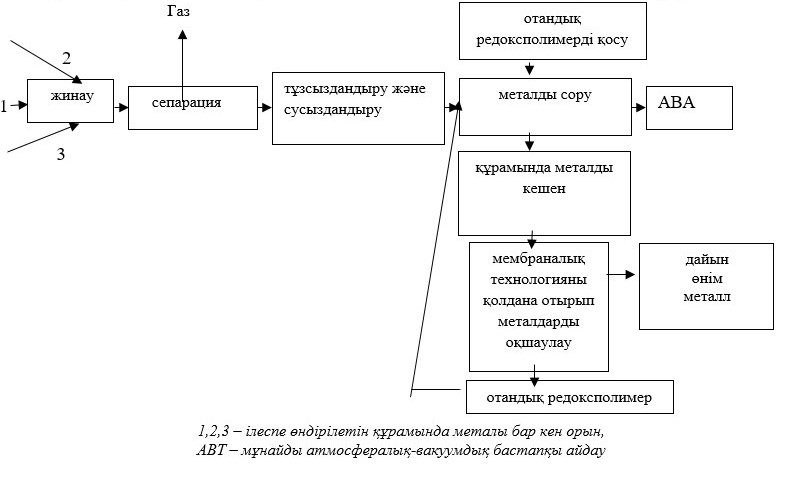
\includegraphics[width=0.8\textwidth]{media/gor/image21.2}
	\caption*{1-сурет. Ілеспе өндірілетін металдарды шығарумен мұнайды жинау
  мен дайындаудың инновациялық технологиялық сұлбасы}
\end{figure}

\begin{multicols}{2}

1-суретте сирек металдарды отандық редоксполимермен және мембраналық
технологиямен шығарып, мұнай мен газ, сонымен қатар мұнай өнімдерін
жинау мен дайындаудың жалпы технологиялық сұлбасы көрсетілген. Қорыта
айтқанда, бұл әдістің негізінде мұнай-газ саласында отандық
редоксполимер негізінде мұнай мен мұнай өнімдерінен ванадий мен басқа
металдарды алу үшін сорбциялық процестерді, сонымен қатар, асыл газдарды
(гелий) бөлу кезінде мембраналық технологияны енгізу ұсынылады. Бұл
мұнай кен орындарын кешенді игеру, мұнай сапасын арттыру және оны өндіру
орындарынан тұтынушыға дейін тасымалдау тиімділігінің талаптарына сәйкес
келеді.

{\bfseries Қорытынды.}

1.Ұсынылған өндіру әдісін талдау нәтижесінде автор қарастырылып отырған
технология қабаттардың мұнай бергіштік коэффициентін арттыруға, сонымен
қатар, қабат пен онымен байланысты металдардан мұнай алу кезінде отандық
редоксполимерді қолдану аясын кеңейтуге мүмкіндігі қарасытырылды. Мұнай
өндірудің гравитациялық режимін және оны кеуектер мен жарықтардан
сорбциялауды қамтамасыз ететін отандық редоксполимер ерітінділерін
қабатқа айдау үшін өндіру және қосалқы ұңғымаларды орналастырудың
технологиялық сұлбасын ұсынылды.

2.Мұнай мен мұнай өнімдерінен, сондай-ақ, газ кен орындарын игеру
кезінде бағалы газдардан (гелий және т.б.) ілеспе өндірілетін ванадий
мен басқа металдарды алудың инновациялық тәсілі негізінде мұнай-газ
саласында отандық редоксполимер негізінде мұнай мен мұнай өнімдерінен
ванадий мен басқа металдарды алу үшін сорбциялық процестерді, сондай-ақ,
асыл газдарды бөлу кезінде мембраналық технологияны енгізу қсынылады,
бұл мұнай және газ кен орындарын кешенді игеру, мұнай газының сапасын
және оны өндіру орындарынан тұтынушыға дейін тасымалдау тиімділігін
арттыруға мүмкіндігін талданды.

3.Мақалада қарастырылған талдау, яғни сұйық ортадан, соның ішінде
мұнайлы қабаттар мен қалдық мұнай қорларын металдарды алу процестерін
зерттеуде ғылымның дамуына үлес қосады.

4.Мұнай мен газдың құнын бағалау кезінде осы уақытқа дейін мұнай мен
газға кіретін басқа да ілеспе өндірілетін пайдалы қазбалардың құнын
есепке алмай, көмірсутектердің болуы ғана ескерілді. Мұнай және газ кен
орындарын кешенді игеру кезінде баға белгілеу кезінде мұнай мен газдың
құнын келтірілген формула бойынша есептеулер жүргізуге болады.
\end{multicols}

\begin{center}
  {\bfseries Әдебиеттер}
  \end{center}
  \begin{references}


1. Li Wang, Jixiang Guo, Chi Li, Ruiying Xiong, Xiangwei Chen, Xiaojun
Zhang Advancements and future prospects in in-situ catalytic technology
for heavy oil reservoirs in China: A review//Fuel. -2024. -Vol. 374.
DOI: 10.1016/j.fuel.2024.132376

2. G. Todd Ventura, Louise Gall, Christopher Siebert, Julie Prytulak,
Peter Szatmari, Martin Hürlimann, Alex N. Halliday The stable isotope
composition of vanadium, nickel, and molybdenum in crude oils//\\Applied
Geochemistry. -2015. -Vol.59. -P. 104-117. DOI:
10.1016/j.apgeochem.2015.04.009

3. Augustine Okeke An exploration of sustainability and supply chain
management practises in the oil and gas industry: A systematic review of
practises and implications//Environmental and Sustainability Indicators.
-2024. -Vol. 23. DOI: 10.1016/j.indic.2024.100462

4. Hadi Sahebi, Farnaz Barzinpour, Hani Gilani Bibliometric analysis of
sustainable supply chain \\management in the oil and gas industry: A
review and research agenda//The Extractive Industries and Society.
-2024. -Vol. 18. DOI: 10.1016/j.exis.2024.101483

5.Нефтедобыча, газификация и привлечение инвестиций --- как развивалась
энергетическая отрасль Казахстана в условиях пандемии. 05 Март
2021//Официальный информационный ресурс Премьер-Министра Республики
Казахстан. 
URL:
\href{https://primeminister.kz/ru/news/neftedobycha-gazifikaciya-i-privlechenie-investiciy-kak-razvivalas-energeticheskaya-otrasl-kazahstana-v-usloviyah-pandemii-52034}{https://primeminister.kz/ru}
(Қаралған күні: 02.09.2024)

6. Виктор Катона Нефть и газ Каспийского региона между Европой и Азией.
17 августа 2017. Аналитические статьи. URL:
\href{https://russiancouncil.ru/analytics-and-comments/analytics/neft-i-gaz-kaspiyskogo-regiona-mezhdu-evropoy-i-aziey/}{https://russiancouncil.ru/analytics-and-comments}
(Қаралған күні: 02.09.2024)

7. Пономарева Г.А. Металлы в нефти месторождений Оренбургской области
//Известия Уральского государственного горного университета. -2019.
-Вып. 2(54). -С. 56-62. DOI: 10.21440/2307-2091-2019-2-56-62.

8. Тагиев Ш. Трудноизвлекаемые запасы нефти и проблемы их добычи:
Увеличение нефтеотдачи трудноизвлекаемых запасов нефти и проблема их
добычи // Мировая наука. -2023. -№6(75). -С.120-124. URL:
\href{https://cyberleninka.ru/article/n/trudnoizvlekaemye-zapasy-nefti-i-problemy-ih-dobychi-uvelechenie-nefteotdachi-trudnoizvlekaemyh-zapasov-nefti-i-problema-ih-dobychi/viewer}{https://cyberleninka.ru}

9. Надиров Н.К., Котова А.В., Камьянов В.Ф. и др. Металлы в нефтях Новые
нефти Казахстана и их использование: Металлы в нефтях: монография.
-Алма-Ата: Наука, 1984. 448 с.

10. Васильянова Л.С. Нефть и газ--богатство Казахстана //Сборник статей
«Геологическая наука независимого Казахстана: достижения и перспективы».
-Алматы, 2011. - С. 282-291.

11. Инновационный патент №25906 на изобретение РК. Инновационный способ
извлечения ванадия из нефти и нефтепродуктов //Ахмеджанов Т.К.,
Нуранбаева Б.М. и др.

12.
\href{https://sbercib.ru/publications/sbercib-investment-research}{Sbercib
investment research: Прогноз цен на золото, серебро, платину и палладий
в 2024 году.} URL:\href{https://sbercib.ru/publication/prognoz-tsen-na-zoloto-serebro-platinu-i-palladii-v-2024-godu}{https://sbercib.ru}
(Қаралған күні: 02.09.2024)

13. International Metallurgical Research Group Мировой рынок редких
металлов по итогам 2023 (апрель 2024)/Рынок ванадия и соединений,
прогноз 2025 Metal Research (Металлургические исследования) URL:
\url{https://www.metalresearch.ru/vanadium_market.html} (Қаралған күні:
02.09.2024)

14. M. Baritto, A.O. Oni, A. Kum The development of a techno-economic
model for the assessment of vanadium recovery from bitumen upgrading
spent catalyst/ Journal of Cleaner Production. -2022. -Vol.363.
\href{https://doi.org/10.1016/j.jclepro.2022.132376}{DOI:10.1016/j.jclepro.2022.132376}

15.Казахстанская еженедельная газета/Kazakh weekly. URL:
newspaper/2012-08-24/ 

\href{https://panoramakz.com/index.php/economics/oil/item/32263-?utm_source=google.com&utm_medium=organic&utm_campaign=google.com&utm_referrer=google.com}{https://panoramakz.com}
(Қаралған күні: 02.09.2024)

16.Nuranbayeva B.M. Method for extraction of vanadium from oil during
preparation //International journal of chemical sciences
(Int.J/Chem.Sci.) -2013. --Vol.11(1). -P.73-84.

17. Ахмеджанов Т.К., Нуранбаева Б.М., Гусенов И.Ш. Повышение нефтеотдачи
пласта с использованием новых отечественных полимеров //Журнал «Нефть и
газ». -- 2015. - № 2 (86). -С. 61-70.

18. Ахмеджанов Т.К., Нуранбаева Б.М. Инновационные способы кучного
выщелачивания золотосодержащих и урановых руд в открытых горных
выра-ботках//Международная научно-практическая конференция «50 лет
российской научной школе комплексного освоения недр земли» Москва, РФ
13-16 ноября 2017. ИПКОН. С.443-447.

19. Ахмеджанов Т.К., Елефтериади Д.К. Исследование альтернативных
методов повышения нефтеотдачи высоковязких нефтей и нефтебитумов
//Поиск. -2019. -№ 2. -С. 136-139.

20. Ахмеджанов Т.К., Нуранбаева Б.М. Cпособ и технологические схемы
извлечения ванадия и других металлов из нефти и нефтепродуктов при их
подготовке //Журнал "Современные наукоёмкие технологии. -- 2013. -- № 4.
-- С. 49-52. URL:
\url{https://top-technologies.ru/ru/article/view?id=31603}
\end{references}

\begin{center}
  {\bfseries References}
  \end{center}
  \begin{references}


1. Li Wang, Jixiang Guo, Chi Li, Ruiying Xiong, Xiangwei Chen, Xiaojun
Zhang Advancements and future prospects in in-situ catalytic technology
for heavy oil reservoirs in China: A review//Fuel. -2024. -Vol. 374.
DOI: 10.1016/j.fuel.2024.132376

2. G. Todd Ventura, Louise Gall, Christopher Siebert, Julie Prytulak,
Peter Szatmari, Martin Hürlimann, Alex N. Halliday The stable isotope
composition of vanadium, nickel, and molybdenum in crude oils//

Applied Geochemistry. -2015. -Vol.59. -P. 104-117. DOI:
10.1016/j.apgeochem.2015.04.009

3. Augustine Okeke An exploration of sustainability and supply chain
management practises in the oil and gas industry: A systematic review of
practises and implications//Environmental and Sustainability Indicators.
-2024. -Vol. 23. DOI: 10.1016/j.indic.2024.100462

4. Hadi Sahebi, Farnaz Barzinpour, Hani Gilani Bibliometric analysis of
sustainable supply chain \\management in the oil and gas industry: A
review and research agenda//The Extractive Industries and Society.
-2024. -Vol. 18. DOI: 10.1016/j.exis.2024.101483

5.Neftedobycha, gazifikacija i privlechenie investicij --- kak
razvivalas'{} jenergeticheskaja otrasl'{}
Kazahstana v uslovijah pandemii. 05 Mart
2021//Oficial' nyj informacionnyj resurs
Prem' er-Ministra Respubliki Kazahstan. URL:
\href{https://primeminister.kz/ru/news/neftedobycha-gazifikaciya-i-privlechenie-investiciy-kak-razvivalas-energeticheskaya-otrasl-kazahstana-v-usloviyah-pandemii-52034}{https://primeminister.kz}
(date of application: 02.09.2024) {[}in Russian{]}

6. Viktor Katona Neft'{} i gaz Kaspijskogo regiona mezhdu
Evropoj i Aziej. 17 avgusta 2017. Analiticheskie stat' i.
URL:
https://russiancouncil.ru/analytics-and-comments/analytics/neft-i-gaz-kaspiyskogo-regiona-mezhdu-evropoy-i-aziey/
(date of application: 02.09.2024) {[}in Russian{]}

7. Ponomareva G.A. Metally v nefti mestorozhdenij Orenburgskoj oblasti
//Izvestija Ural' skogo \\gosudarstvennogo gornogo
universiteta. -2019. -Vol. 2(54). -S. 56-62. DOI:
10.21440/2307-2091-2019-2-56-62. {[}in Russian{]}

8. Tagiev Sh. Trudnoizvlekaemye zapasy nefti i problemy ih dobychi:
Uvelichenie nefteotdachi \\trudnoizvlekaemyh zapasov nefti i problema ih
dobychi // Mirovaja nauka. -2023. -№6(75). -S.120-124. URL:
\href{https://cyberleninka.ru/article/n/trudnoizvlekaemye-zapasy-nefti-i-problemy-ih-dobychi-uvelechenie-nefteotdachi-trudnoizvlekaemyh-zapasov-nefti-i-problema-ih-dobychi/viewer}{https://cyberleninka.ru}
{[}in Russian{]}

9. Nadirov N.K., Kotova A.V., Kam' janov V.F. i dr.
Metally v neftjah Novye nefti Kazahstana i ih
ispol' zovanie: Metally v neftjah: monografija.
-Alma-Ata: Nauka, 1984. 448 s. {[}in Russian{]}

10. Vasil' janova L.S. Neft'{} i
gaz--bogatstvo Kazahstana //Sbornik statej «Geologicheskaja nauka

nezavisimogo Kazahstana: dostizhenija i perspektivy». -Almaty, 2011. -
S. 282-291. {[}in Russian{]}

11. Innovacionnyj patent №25906 na izobretenie RK. Innovacionnyj sposob
izvlechenija vanadija iz nefti i nefteproduktov //Ahmedzhanov T.K.,
Nuranbaeva B.M. i dr. {[}in Russian{]}

12. Sbercib investment research: Prognoz cen na zoloto, serebro, platinu
i palladij v 2024 godu. URL:
\href{https://sbercib.ru/publication/prognoz-tsen-na-zoloto-serebro-platinu-i-palladii-v-2024-godu}{https://sbercib.ru}
(date of application: 02.09.2024) {[}in Russian{]}

13. International Metallurgical Research Group Mirovoj rynok redkih
metallov po itogam 2023 (aprel'{} 2024)/Rynok vanadija i
soedinenij, prognoz 2025 Metal Research (Metallurgicheskie
issledovanija) URL: https://www.metalresearch.ru/vanadium\_market.html
(date of application: 02.09.2024)

14. M. Baritto, A.O. Oni, A. Kum The development of a techno-economic
model for the assessment of vanadium recovery from bitumen upgrading
spent catalyst/ Journal of Cleaner Production. -2022. -Vol.363.
DOI:10.1016/j.jclepro.2022.132376

15.Kazahstanskaja ezhenedel' naja gazeta/Kazakh weekly.
URL: newspaper/2012-08-24/

\href{https://panoramakz.com/index.php/economics/oil/item/32263-?utm\_source=google.com\&utm\_medium=organic\&utm\_campaign=google.com\&utm\_referrer=google.com}{https://panoramakz.com}
(date of application: 02.09.2024) {[}in Russian{]}

16.Nuranbayeva B.M. Method for extraction of vanadium from oil during
preparation //International journal of chemical sciences
(Int.J/Chem.Sci.) -2013. --Vol.11(1). -P.73-84.

17. Ahmedzhanov T.K., Nuranbaeva B.M., Gusenov I.Sh. Povyshenie
nefteotdachi plasta s ispol' zovaniem novyh
otechestvennyh polimerov //Zhurnal «Neft'{} i gaz». --
2015. - № 2 (86). -S. 61-70. {[}in Russian{]}

18. Ahmedzhanov T.K., Nuranbaeva B.M. Innovacionnye sposoby kuchnogo
vyshhelachivanija \\zolotosoderzhashhih i uranovyh rud v otkrytyh gornyh
vyra-botkah//Mezhdunarodnaja nauchno-

prakticheskaja konferencija «50 let
rossijskoj nauchnoj shkole kompleksnogo osvoenija nedr zemli» Moskva, RF
13-16 nojabrja 2017. IPKON. S.443-447. {[}in Russian{]}

19. Ahmedzhanov T.K., Elefteriadi D.K. Issledovanie
al' ternativnyh metodov povyshenija nefteotdachi
vysokovjazkih neftej i neftebitumov //Poisk. -2019. -№ 2. -S. 136-139.
{[}in Russian{]}

20. Ahmedzhanov T.K., Nuranbaeva B.M. Cposob i tehnologicheskie shemy
izvlechenija vanadija i drugih metallov iz nefti i nefteproduktov pri ih
podgotovke //Zhurnal "Sovremennye naukojomkie tehnologii. -- 2013. -- №
4. -- S. 49-52. URL:
\url{https://top-technologies.ru/ru/article/view?id=31603} {[}in
Russian{]}
\end{references}


\begin{authorinfo}
  \hspace{1em}\emph{{\bfseries Сведения об авторе}}

Нуранбаева Б.М. - канд.хим.наук, ассоциированный профессор, лидер
программ образовательной программы «Нефтяная инженерия» и «Горное и
нефтегазовое дело» Института Инженерии, Caspian University, Алматы,
Казахстан, e-mail: bulbulmold@mail.ru

\hspace{1em}\emph{{\bfseries Information about the author}}

Nuranbaeva B.M. - Candidate of Chemical Sciences, Associate Professor, Program Leader of Educational Program
“Petroleum Engineering” and “Mining and Oil and Gas Engineering”, Institute of Engineering, Caspian University,
Almaty, Kazakhstan, e-mail: bulbulmold@mail.ru.
\end{authorinfo}

